% Gradient Info
  
\tikzset {_4gmy02s9w/.code = {\pgfsetadditionalshadetransform{ \pgftransformshift{\pgfpoint{0 bp } { 0 bp }  }  \pgftransformrotate{-90 }  \pgftransformscale{2 }  }}}
\pgfdeclarehorizontalshading{_a2s7rjldk}{150bp}{rgb(0bp)=(0.52,0.7,0.83);
rgb(37.5bp)=(0.52,0.7,0.83);
rgb(37.589285714285715bp)=(0.65,0.78,0.86);
rgb(100bp)=(0.65,0.78,0.86)}

% Gradient Info
  
\tikzset {_47vd44iuy/.code = {\pgfsetadditionalshadetransform{ \pgftransformshift{\pgfpoint{0 bp } { 0 bp }  }  \pgftransformrotate{-90 }  \pgftransformscale{2 }  }}}
\pgfdeclarehorizontalshading{_lr3lb1pkn}{150bp}{rgb(0bp)=(0.52,0.7,0.83);
rgb(37.5bp)=(0.52,0.7,0.83);
rgb(37.589285714285715bp)=(0.65,0.78,0.86);
rgb(100bp)=(0.65,0.78,0.86)}

% Gradient Info
  
\tikzset {_7sudtrh7o/.code = {\pgfsetadditionalshadetransform{ \pgftransformshift{\pgfpoint{0 bp } { 0 bp }  }  \pgftransformrotate{-90 }  \pgftransformscale{2 }  }}}
\pgfdeclarehorizontalshading{_58d2mupl3}{150bp}{rgb(0bp)=(0.52,0.7,0.83);
rgb(37.5bp)=(0.52,0.7,0.83);
rgb(37.589285714285715bp)=(0.65,0.78,0.86);
rgb(100bp)=(0.65,0.78,0.86)}

% Gradient Info
  
\tikzset {_8yw1knx6e/.code = {\pgfsetadditionalshadetransform{ \pgftransformshift{\pgfpoint{0 bp } { 0 bp }  }  \pgftransformrotate{-90 }  \pgftransformscale{2 }  }}}
\pgfdeclarehorizontalshading{_wvcs4u4to}{150bp}{rgb(0bp)=(0.52,0.7,0.83);
rgb(37.5bp)=(0.52,0.7,0.83);
rgb(37.589285714285715bp)=(0.65,0.78,0.86);
rgb(100bp)=(0.65,0.78,0.86)}

% Gradient Info
  
\tikzset {_5okmrbah7/.code = {\pgfsetadditionalshadetransform{ \pgftransformshift{\pgfpoint{0 bp } { 0 bp }  }  \pgftransformrotate{-90 }  \pgftransformscale{2 }  }}}
\pgfdeclarehorizontalshading{_1514r63hw}{150bp}{rgb(0bp)=(0.89,0.89,0.89);
rgb(62.5bp)=(0.89,0.89,0.89);
rgb(62.5bp)=(0.86,0.86,0.86);
rgb(62.5bp)=(0.82,0.82,0.82);
rgb(100bp)=(0.82,0.82,0.82)}

% Gradient Info
  
\tikzset {_parm60zdm/.code = {\pgfsetadditionalshadetransform{ \pgftransformshift{\pgfpoint{0 bp } { 0 bp }  }  \pgftransformrotate{-90 }  \pgftransformscale{2 }  }}}
\pgfdeclarehorizontalshading{_qtarayl0h}{150bp}{rgb(0bp)=(0.89,0.89,0.89);
rgb(62.5bp)=(0.89,0.89,0.89);
rgb(62.5bp)=(0.86,0.86,0.86);
rgb(62.5bp)=(0.82,0.82,0.82);
rgb(100bp)=(0.82,0.82,0.82)}

% Gradient Info
  
\tikzset {_6rcrm5w80/.code = {\pgfsetadditionalshadetransform{ \pgftransformshift{\pgfpoint{0 bp } { 0 bp }  }  \pgftransformrotate{-90 }  \pgftransformscale{2 }  }}}
\pgfdeclarehorizontalshading{_h63rtflmc}{150bp}{rgb(0bp)=(0.89,0.89,0.89);
rgb(62.5bp)=(0.89,0.89,0.89);
rgb(62.5bp)=(0.86,0.86,0.86);
rgb(62.5bp)=(0.82,0.82,0.82);
rgb(100bp)=(0.82,0.82,0.82)}

% Gradient Info
  
\tikzset {_lqvsggp8q/.code = {\pgfsetadditionalshadetransform{ \pgftransformshift{\pgfpoint{0 bp } { 0 bp }  }  \pgftransformrotate{-90 }  \pgftransformscale{2 }  }}}
\pgfdeclarehorizontalshading{_mk3p3cfhk}{150bp}{rgb(0bp)=(0.89,0.89,0.89);
rgb(62.5bp)=(0.89,0.89,0.89);
rgb(62.5bp)=(0.86,0.86,0.86);
rgb(62.5bp)=(0.82,0.82,0.82);
rgb(100bp)=(0.82,0.82,0.82)}

% Gradient Info
  
\tikzset {_dctjay13h/.code = {\pgfsetadditionalshadetransform{ \pgftransformshift{\pgfpoint{0 bp } { 0 bp }  }  \pgftransformrotate{-90 }  \pgftransformscale{2 }  }}}
\pgfdeclarehorizontalshading{_yzcd0ijfo}{150bp}{rgb(0bp)=(0.89,0.89,0.89);
rgb(62.5bp)=(0.89,0.89,0.89);
rgb(62.5bp)=(0.86,0.86,0.86);
rgb(62.5bp)=(0.82,0.82,0.82);
rgb(100bp)=(0.82,0.82,0.82)}
\tikzset{every picture/.style={line width=0.75pt}} %set default line width to 0.75pt        

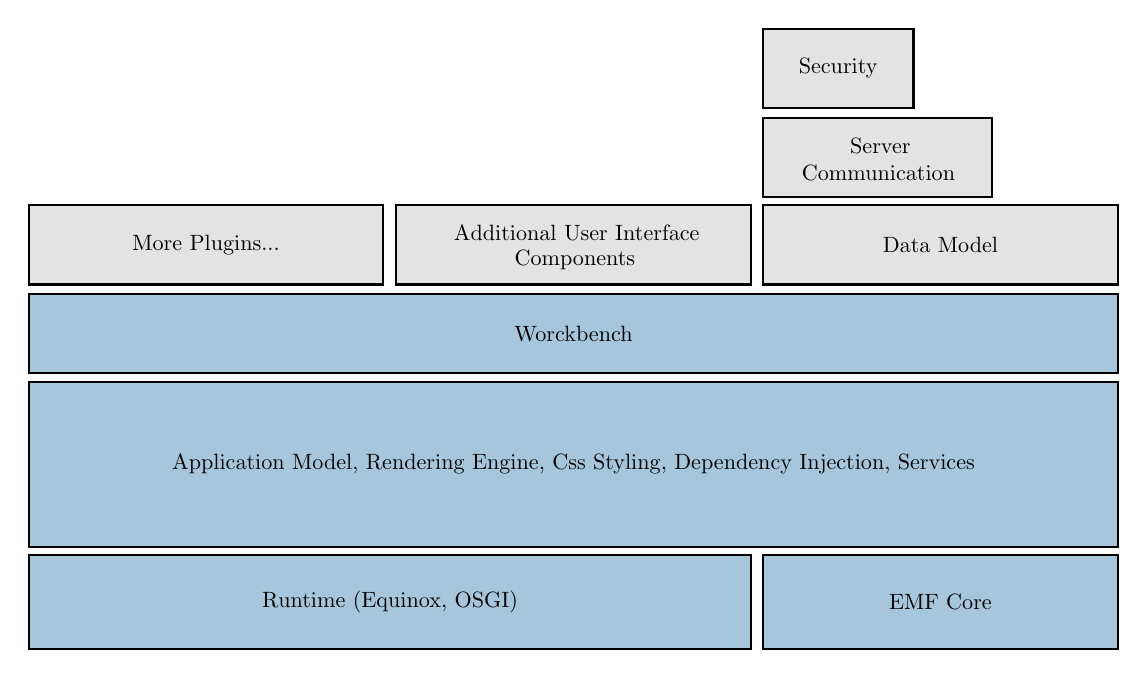
\begin{tikzpicture}[x=0.75pt,y=0.75pt,yscale=-1,xscale=1]
%uncomment if require: \path (0,451); %set diagram left start at 0, and has height of 451


%Shape: Rectangle [id:dp7026166067585526] 
\path  [shading=_a2s7rjldk,_4gmy02s9w] (3.5,256.57) -- (351.71,256.57) -- (351.71,302) -- (3.5,302) -- cycle ; % for fading 
 \draw   (3.5,256.57) -- (351.71,256.57) -- (351.71,302) -- (3.5,302) -- cycle ; % for border 

%Shape: Rectangle [id:dp6345226770671628] 
\path  [shading=_lr3lb1pkn,_47vd44iuy] (357.32,256.57) -- (528.22,256.57) -- (528.22,302) -- (357.32,302) -- cycle ; % for fading 
 \draw   (357.32,256.57) -- (528.22,256.57) -- (528.22,302) -- (357.32,302) -- cycle ; % for border 

%Shape: Rectangle [id:dp04645949367639268] 
\path  [shading=_58d2mupl3,_7sudtrh7o] (3.5,173.17) -- (528.5,173.17) -- (528.5,252.56) -- (3.5,252.56) -- cycle ; % for fading 
 \draw   (3.5,173.17) -- (528.5,173.17) -- (528.5,252.56) -- (3.5,252.56) -- cycle ; % for border 

%Shape: Rectangle [id:dp28788690760284585] 
\path  [shading=_wvcs4u4to,_8yw1knx6e] (3.5,130.92) -- (528.5,130.92) -- (528.5,169.08) -- (3.5,169.08) -- cycle ; % for fading 
 \draw   (3.5,130.92) -- (528.5,130.92) -- (528.5,169.08) -- (3.5,169.08) -- cycle ; % for border 

%Shape: Rectangle [id:dp8477585057798736] 
\path  [shading=_1514r63hw,_5okmrbah7] (3.5,88.08) -- (174.4,88.08) -- (174.4,126.24) -- (3.5,126.24) -- cycle ; % for fading 
 \draw   (3.5,88.08) -- (174.4,88.08) -- (174.4,126.24) -- (3.5,126.24) -- cycle ; % for border 

%Shape: Rectangle [id:dp9553905279309911] 
\path  [shading=_qtarayl0h,_parm60zdm] (357.32,88.08) -- (528.22,88.08) -- (528.22,126.24) -- (357.32,126.24) -- cycle ; % for fading 
 \draw   (357.32,88.08) -- (528.22,88.08) -- (528.22,126.24) -- (357.32,126.24) -- cycle ; % for border 

%Shape: Rectangle [id:dp8432494375409605] 
\path  [shading=_h63rtflmc,_6rcrm5w80] (180.41,88.08) -- (351.31,88.08) -- (351.31,126.24) -- (180.41,126.24) -- cycle ; % for fading 
 \draw   (180.41,88.08) -- (351.31,88.08) -- (351.31,126.24) -- (180.41,126.24) -- cycle ; % for border 
%Shape: Rectangle [id:dp23364015098761448] 
\path  [shading=_mk3p3cfhk,_lqvsggp8q] (357.2,45.95) -- (467.47,45.95) -- (467.47,84.11) -- (357.2,84.11) -- cycle ; % for fading 
 \draw   (357.2,45.95) -- (467.47,45.95) -- (467.47,84.11) -- (357.2,84.11) -- cycle ; % for border 


%Shape: Rectangle [id:dp4202456795602847] 
\path  [shading=_yzcd0ijfo,_dctjay13h] (357.2,3) -- (429.78,3) -- (429.78,41.16) -- (357.2,41.16) -- cycle ; % for fading 
 \draw   (357.2,3) -- (429.78,3) -- (429.78,41.16) -- (357.2,41.16) -- cycle ; % for border 


% Text Node
\draw (266,212.86) node [scale=0.8] [align=left] {Application Model, Rendering Engine, Css Styling, Dependency Injection, Services};
% Text Node
\draw (177.6,279.29) node [scale=0.8] [align=left] {Runtime (Equinox, OSGI)};
% Text Node
\draw (442.77,279.29) node [scale=0.8] [align=left] {EMF Core};
% Text Node
\draw (266,150) node [scale=0.8] [align=left] {Worckbench};
% Text Node
\draw (88.95,107.16) node [scale=0.8] [align=left] {More Plugins...};
% Text Node
\draw (267.54,101.49) node [scale=0.8] [align=left] {Additional User Interface};
% Text Node
\draw (266.64,114.46) node [scale=0.8] [align=left] {Components};
% Text Node
\draw (442.77,107.16) node [scale=0.8] [align=left] {Data Model};
% Text Node
\draw (413.82,59.36) node [scale=0.8] [align=left] {Server};
% Text Node
\draw (412.93,72.32) node [scale=0.8] [align=left] {Communication};
% Text Node
\draw (393.49,22.08) node [scale=0.8] [align=left] {Security};


\end{tikzpicture}